\begin{figure}
   \centering
   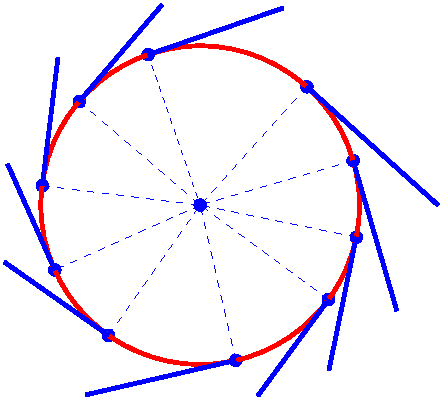
\includegraphics[width=7.5cm]{Cfamd_1.pdf}
   \caption{question 1}
\end{figure}
\begin{figure}
   \centering
   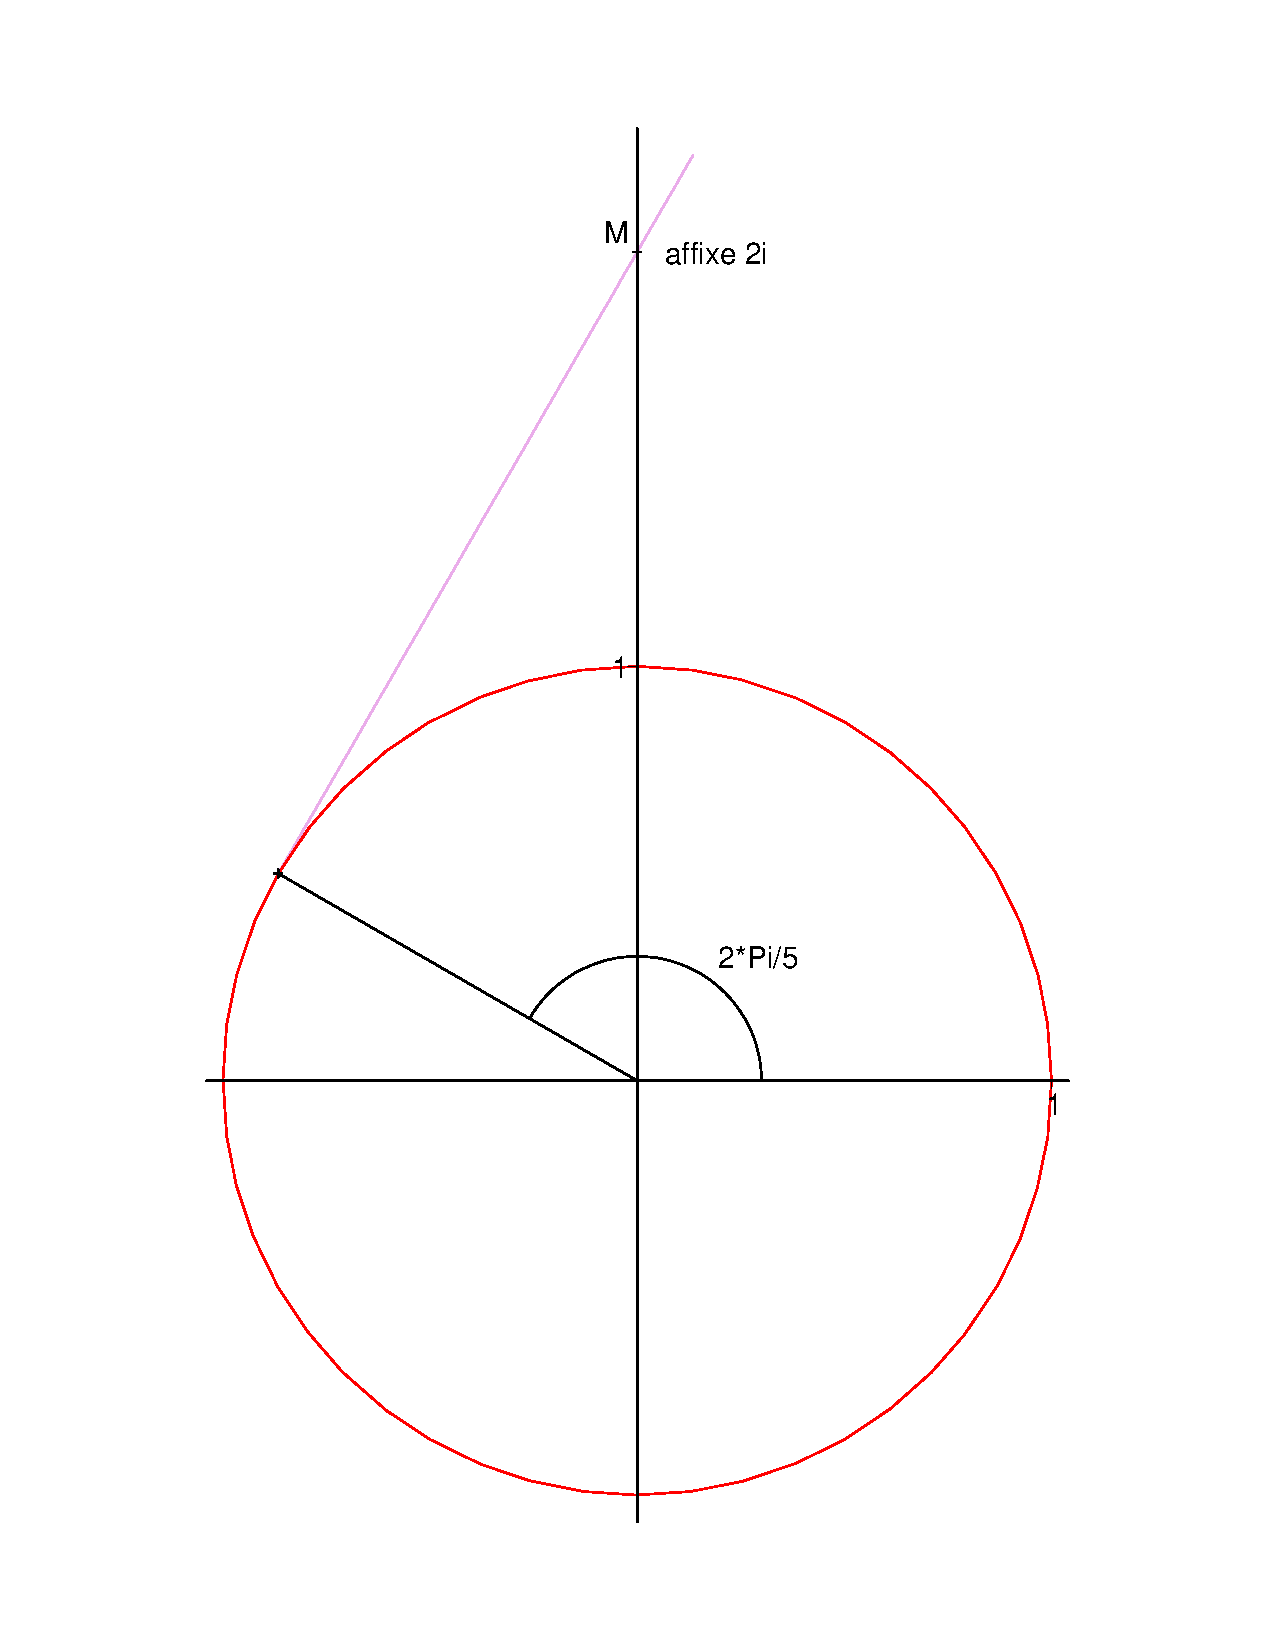
\includegraphics[scale=0.25]{Cfamd_2.pdf}
   \caption{question 4}
\end{figure}
\begin{enumerate}
\item L'ensemble $D(t)$ est la demi-droite d'extrémité le point $T(t)$ d'affixe $e^{it}$ et de direction le vecteur d'affixe $e^{i(t-\frac{\Pi}{2})}$. Cette demi-droite est clairement tangente en $T(t)$ au cercle de centre $O$ et de rayon 1.
\item Comme $r$ est positif, la relation
\[1-\lambda i = r e^{i(t-\frac{\Pi}{2})}\]
entraîne que $r = \vert 1-\lambda i \vert=\sqrt{1+\lambda^2}$.\newline
Lorsque la partie réelle d'un nombre complexe est strictement positive, un de ses arguments est l'$\arctan$ du quotient de sa partie imaginaire sur sa partie réelle. C'est bien le cas ici, on en déduit
\[-arctan(\lambda)=\theta -t \quad (2\pi)\]
puis
\begin{eqnarray*}
\lambda = \sqrt{r^2-1}\\
 t = \theta + \arctan(\sqrt{r^2-1})\quad (2\pi)
\end{eqnarray*}
\item Soit $M$ un point d'affixe $r e^{i(\theta)}$ avec $r\geq 1$ (en dehors du disque). Supposons que, pour un certain $t$, $M\in D(t)$. Il existe alors un $\lambda \geq 0$ tel que
\[re^{i\theta}=e^{it}+\lambda e^{i(t-\frac{\pi}{2})}\]
Après division par $e^{it}$, cette relation devient
\[re^{i(\theta - t)}=1-\lambda i\]
D'après la question précédente, il existe un seul $\lambda$ positif (qui vaut $\sqrt{r^2 -1}$) et une infinité de $t$ tous congrus modulo $2\pi$ à $\theta + \arctan(\sqrt{r^2-1})$. Lorsque deux valeurs de $t$ sont congrues modulo $2\pi$, elles définissent la même demi-droite. Il existe donc une seule demi-droite qui contient le point $M$.
\item Pour $M$ d'affixe $2i$, $r=2$ et $\theta = \frac{\pi}{2}$ donc $\lambda=\sqrt{3}$. Comme $\cos(\frac{\pi}{3})=\frac{1}{2}$ et $\sin(\frac{\pi}{3})=\frac{\sqrt{3}}{2}$, $\arctan(\sqrt{3})=\frac{\pi}{3}$ et $t= \frac{\pi}{2}-\frac{\pi}{3}=\frac{5\pi}{6}$.
\item On vient de montrer que $M$ d'affixe $2i$ est sur l'unique demi-droite $D(\frac{5\pi}{6})$. Un vecteur directeur de cette demi-droite fait avec l'axe des $x$ un angle $\frac{5\pi}{6}-\frac{\pi}{2}=\frac{\pi}{3}$.\newline
D'autre part, $r=2$, $\theta=\frac{\pi}{2}$. Donc
\[(1+i\sqrt{r^2-1})e^{i\theta}=(1+i\sqrt{3})i=2e^{i(\frac{\pi}{3}-\frac{\pi}{2})}\]
Ceci prouve bien que (dans ce cas particulier) le vecteur d'affixe
\[(1+i\sqrt{r^2-1})e^{i\theta}\]
est orthogonal à un vecteur directeur de $D(t)$ d'affixe $e^{i\frac{\pi}{3}}$.\newline
Plus généralement, on a vu que si $M$ d'affixe $re^{i\theta}$. Il est sur une unique demi-droite $D(t)$ son affixe s'écrivant
$e^{it}+\lambda e^{i(t-\frac{\pi}{2})}$ avec $\lambda=\sqrt{r^2 -1}$ et $t= \theta + \arctan(\sqrt{r^2-1})$.
On peut donc encore écrire
\[1+i\sqrt{r^2-1}=re^{-i(\theta-t)}\]
donc
\[(1+i\sqrt{r^2-1})e^{i\theta}=re^{it}\]
qui est bien l'affixe d'un vecteur orthogonal à $D(t)$.
\item
\begin{enumerate}
\item Les règles usuelles de dérivation s'appliquent pour les fonctions à valeurs complexes.
\[M'(r)=e^{i\theta(r)}+ir\theta'(r)e^{i\theta(r)}\]
\item On a vu que si $M(r)=re^{i\theta(r)} \in D(t)$ alors
\[(1+i\sqrt{r^2-1})e^{i\theta}=re^{it}\]
est l'affixe d'un vecteur orthogonal à $D(t)$. Par conséquent $\overrightarrow{m'}(r)$ est othogonal à $D(t)$ lorsque le quotient des affixes est réel. Transformons ce quotient :
\begin{displaymath}
\frac{e^{i\theta}+ir\theta'e^{i\theta}}{(1+i\sqrt{r^2-1})e^{i\theta}}=
\frac{1+ir\theta'}{1+i\sqrt{r^2-1}}=
\frac{(1+ir\theta')(1-i\sqrt{r^2-1})}{\vert 1+i\sqrt{r^2-1}\vert^2} 
\end{displaymath}
Cette expression est réelle lorsque la partie imaginaire du numérateur est nulle c'est à dire
\[r\theta'- \sqrt{r^2-1}=0\]
\end{enumerate}
\end{enumerate}
